\documentclass{standalone}
\usepackage{tikz} 

\begin{document}
	
	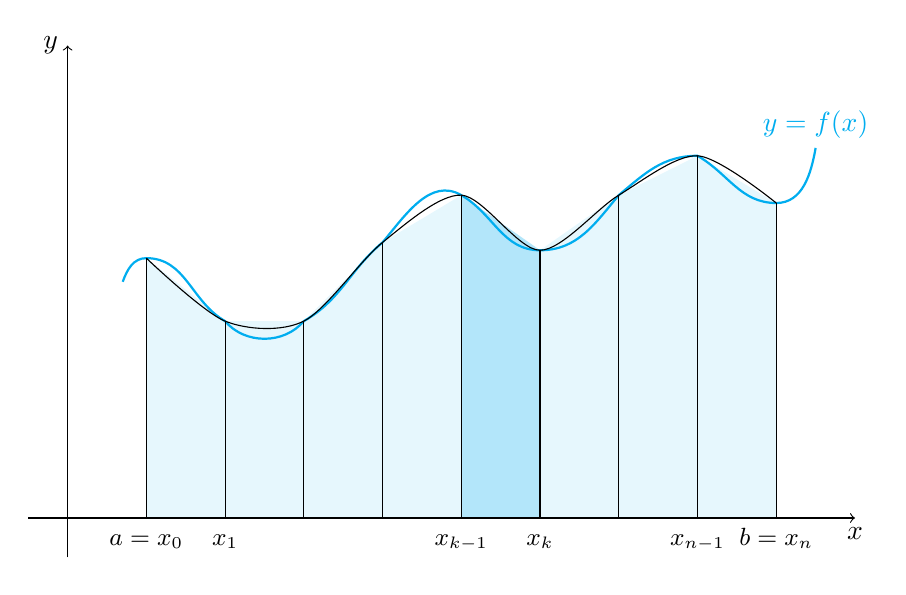
\begin{tikzpicture}
		\coordinate (p1) at (0.7,3);
		\coordinate (p2) at (1,3.3);
		\coordinate (p3) at (2,2.5);
		\coordinate (p4) at (3,2.5);
		\coordinate (p5) at (4,3.5);
		\coordinate (p6) at (5,4.1);
		\coordinate (p7) at (6,3.4);
		\coordinate (p8) at (7,4.1);
		\coordinate (p9) at (8,4.6);
		\coordinate (p10) at (9,4);
		\coordinate (p11) at (9.5,4.7);
		
		% The cyan background
		\fill[cyan!10]
		(p2|-0,0) -- (p2) -- (p3) -- (p4) -- (p5) -- (p6) -- (p7) -- (p8) -- (p9) -- (p10) -- (p10|-0,0) -- cycle;
		% the dark cyan stripe
		\fill[cyan!30] (p6|-0,0) -- (p6) -- (p7) -- (p7|-0,0) -- cycle;
		% the curve
		\draw[thick,cyan]
		(p1) to[out=70,in=180] (p2) to[out=0,in=150]
		(p3) to[out=-50,in=230] (p4) to[out=30,in=220]
		(p5) to[out=50,in=150] (p6) to[out=-30,in=180]
		(p7) to[out=0,in=230] (p8) to[out=40,in=180]
		(p9) to[out=-30,in=180] (p10) to[out=0,in=260] (p11);
		% the broken line connecting points on the curve
		%\draw (p2) parabola (p3) parabola (p4) parabola (p5) parabola (p6) parabola (p7) parabola (p8) parabola (p9) parabola (p10);%Changed
		\draw plot[smooth,samples=9,domain=2:10,variable=\x] (p\x);
		
		% vertical lines and labels
		\foreach \n/\texto in {2/{a=x_0},3/{x_1},4/{},5/{},6/{x_{k-1}},7/{x_k},8/{},9/{x_{n-1}},10/{b=x_n}}
		{
			\draw (p\n|-0,0) -- (p\n);
			\node[below,text height=1.5ex,text depth=1ex,font=\small] at (p\n|-0,0) {$\texto$};
		}
		% The axes
		\draw[->] (-0.5,0) -- (10,0) coordinate (x axis);
		\draw[->] (0,-0.5) -- (0,6) coordinate (y axis);
		% labels for the axes
		\node[below] at (x axis) {$x$};
		\node[left] at (y axis) {$y$};
		% label for the function
		\node[above,text=cyan] at (p11) {$y=f(x)$};
	\end{tikzpicture}
\end{document} 